\documentclass{scrreprt}
\usepackage[a4paper,margin=2.5cm]{geometry}
\usepackage{listings}
\usepackage{underscore}
\usepackage{graphicx}
\usepackage[utf8]{inputenc}
\usepackage[T1]{fontenc}
\usepackage[english]{babel}
\usepackage{booktabs}
\usepackage{longtable}
\usepackage{tabularx}
\usepackage{array}
\usepackage{enumitem}
\usepackage{float}
\usepackage{xcolor}
\usepackage{tikz}
\usetikzlibrary{shapes.multipart,positioning,arrows.meta,calc}
\usepackage[bookmarks=true]{hyperref}
\hypersetup{
    bookmarks=false,
    pdftitle={Software Requirements Specification - BloodLine},
    pdfauthor={Avraj Singh Sekhon, Krish Kumar, Kyna Sood, Manya Sabherwal},
    pdfsubject={Predictive Blood Shortage and Smart Donor Matching Platform},
    pdfkeywords={SRS, BloodLine, blood bank, forecasting, donor matching},
    colorlinks=true,
    linkcolor=blue,
    citecolor=black,
    filecolor=black,
    urlcolor=purple,
    linktoc=page
}%
\def\myversion{1.0 }
\setcounter{tocdepth}{1}
\date{}
\setlength{\parindent}{0pt}
\setlength{\parskip}{0.6em}
\renewcommand{\arraystretch}{1.25}
\renewcommand*{\figureformat}{\figurename~\thefigure}
\renewcommand*{\captionformat}{: }

% requirement-table helpers
\newcolumntype{L}[1]{>{\raggedright\arraybackslash}p{#1}}
\newcommand{\mvp}{MVP}
\newcommand{\incb}{Inc.\,2}

\begin{document}

\begin{flushright}
    \rule{\textwidth}{5pt}\vskip1cm
    \begin{bfseries}
        \Huge{SOFTWARE REQUIREMENTS\\ SPECIFICATION}\\
        \vspace{1.2cm}
        for\\
        \vspace{1.2cm}
        BLOODLINE\\
        \Large{Predictive Blood Shortage and\\ Smart Donor Matching Platform}\\
        \vspace{1.2cm}
        \LARGE{Version \myversion}\\
        \vspace{1.2cm}
        \large
        Prepared by :\\
        1. Avraj Singh Sekhon (1024030287)\\
        2. Krish Kumar (1024030296)\\
        3. Kyna Sood (1024030303)\\
        4. Manya Sabherwal (1024030288)\\
        \vspace{1.2cm}
        Submitted to : Ms. Anushka\\
        Course UCS503P\\
        Thapar Institute of Engineering and Technology\\
        \vspace{1.2cm}
        October 13, 2026\\
    \end{bfseries}
\end{flushright}


\tableofcontents

\chapter{Introduction}

\section{Purpose}
Blood banks and hospitals often find out that a blood group is running low only when the shortage has already started. Stock is tracked, but future demand is not forecast; blood-bank stock, hospital needs and donors are kept in different places; and finding suitable donors by blood group, donation history, distance, availability and consent is slow manual work. So, ``BloodLine'' is the solution.
\newline
``BloodLine'' is a web-based platform which combines inventory tracking, short-term demand forecasting, shortage-risk detection and rule-based donor matching in one role-based system. The main concept of ``BloodLine'' is to change blood availability management from a reactive process into a proactive one. This SRS describes the proposed system of the project proposal for UCS503P.

\section{Intended Audience and Reading Suggestions}
This SRS is for developers, project managers, users, testers and course evaluators. Further the discussion will provide all the internal, external, functional and also non-functional information about ``BloodLine''. Requirements are marked \textbf{MVP} (first iteration) or \textbf{Inc.\,2} (subsequent deliverables).

\section{Project Scope}
``BloodLine'' creates a space for Donors, Blood-Bank Managers, Inventory Staff, Medical Staff, Hospital Coordinators and System Administrators for managing blood availability.
\newline
Inventory staff record the blood stock by blood group and every receipt, issue and expiry. BloodLine forecasts near-term demand from historical data and compares it with the stock. Every blood group gets a LOW, MODERATE or HIGH shortage-risk flag with a plain-English reason.
\newline
The manager reviews the risk and asks BloodLine for matching donors: compatible blood group, past the donation cooldown, available, nearby and with notification consent. Donors are only suggested. Medical staff do the final screening before a donation is recorded.
\newline
Hospital coordinators send blood requests. The manager approves or rejects them, and an approved request issues the units from inventory. The administrator manages accounts and roles.
\newline
BloodLine does not make final medical eligibility decisions and does not move blood between banks. Forecasts are risk signals, not guarantees.

\begin{figure}[H]
    \centering
    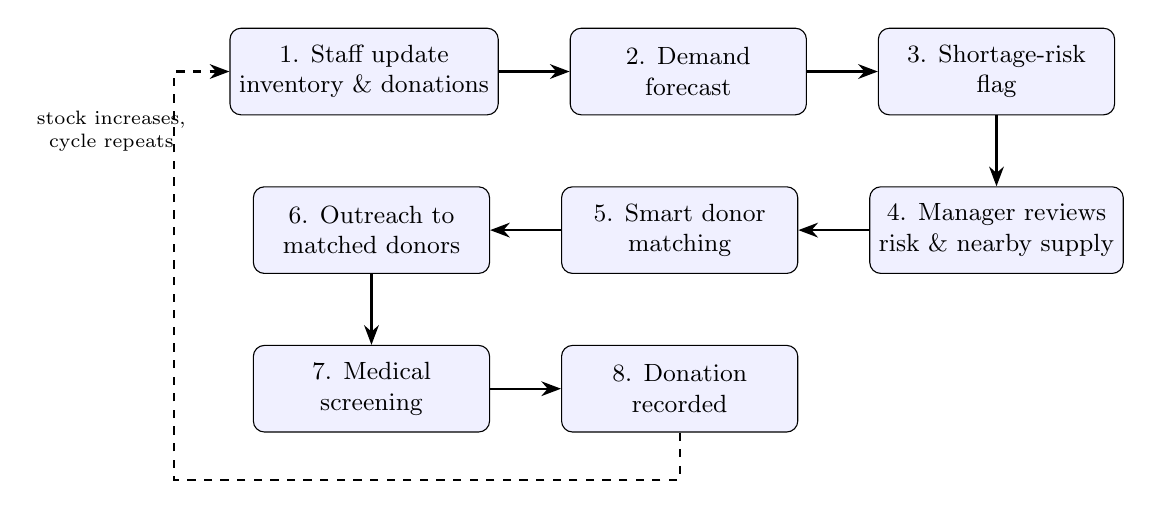
\begin{tikzpicture}[
        box/.style={draw,rounded corners,align=center,minimum width=3.0cm,minimum height=1.1cm,font=\small,fill=blue!6},
        arr/.style={-{Stealth[length=2.5mm]},thick},
        node distance=0.9cm and 0.9cm]
        \node[box] (a) {1. Staff update\\ inventory \& donations};
        \node[box,right=of a] (b) {2. Demand\\ forecast};
        \node[box,right=of b] (c) {3. Shortage-risk\\ flag};
        \node[box,below=of c] (d) {4. Manager reviews\\ risk \& nearby supply};
        \node[box,left=of d] (e) {5. Smart donor\\ matching};
        \node[box,left=of e] (f) {6. Outreach to\\ matched donors};
        \node[box,below=of f] (g) {7. Medical\\ screening};
        \node[box,right=of g] (h) {8. Donation\\ recorded};
        \draw[arr] (a)--(b); \draw[arr] (b)--(c); \draw[arr] (c)--(d);
        \draw[arr] (d)--(e); \draw[arr] (e)--(f); \draw[arr] (f)--(g);
        \draw[arr] (g)--(h);
        \draw[arr,dashed] (h.south) -- ++(0,-0.6) -| ([xshift=-0.7cm]a.west) -- (a.west);
        \node[font=\scriptsize,align=center] at ([xshift=-1.5cm,yshift=-0.2cm]a.south west) {stock increases,\\ cycle repeats};
    \end{tikzpicture}
    \caption{Entire work-flow}
    \label{fig:workflow}
\end{figure}
Figure~\ref{fig:workflow} (Entire work-flow) is the overview of the project. Connection of all the entities are dependable to each other. This gives the simple idea about the functional activities of the project.
\newline
Inventory cycle, in Figure~\ref{fig:workflow}: ``Staff'' update ``Inventory''; BloodLine ``forecasts'' and raises a ``risk flag''; the ``Manager'' reviews it.
\newline
Donor cycle, in Figure~\ref{fig:workflow}: the ``Manager'' asks for ``matches''; ``Donors'' are contacted; ``Medical staff'' screen them; the ``Donation'' is recorded and stock rises.

\chapter{Overall Description}

\section{Product Perspective}
``BloodLine'' is the replacement of the manual and scattered blood availability process. Stock registers, donor lists and request slips are kept in one system. Main goal of this project is to minimize the time needed to find and respond to a shortage. It is a new web application with a 3-tier architecture (Figure~\ref{fig:arch}).

\begin{figure}[H]
    \centering
    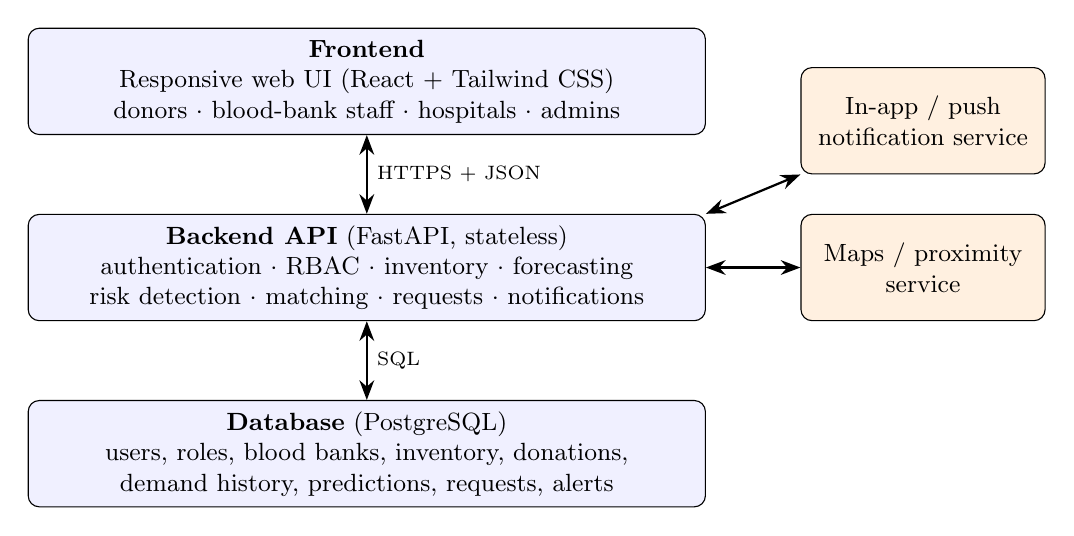
\begin{tikzpicture}[
        layer/.style={draw,rounded corners,align=center,minimum width=8.6cm,minimum height=1.35cm,font=\small,fill=blue!6},
        ext/.style={draw,rounded corners,align=center,minimum width=3.1cm,minimum height=1.35cm,font=\small,fill=orange!12},
        arr/.style={{Stealth[length=2.5mm]}-{Stealth[length=2.5mm]},thick}]
        \node[layer] (fe) {\textbf{Frontend}\\ Responsive web UI (React + Tailwind CSS)\\ donors $\cdot$ blood-bank staff $\cdot$ hospitals $\cdot$ admins};
        \node[layer,below=1cm of fe] (be) {\textbf{Backend API} (FastAPI, stateless)\\ authentication $\cdot$ RBAC $\cdot$ inventory $\cdot$ forecasting\\ risk detection $\cdot$ matching $\cdot$ requests $\cdot$ notifications};
        \node[layer,below=1cm of be] (db) {\textbf{Database} (PostgreSQL)\\ users, roles, blood banks, inventory, donations,\\ demand history, predictions, requests, alerts};
        \node[ext,right=1.2cm of be] (map) {Maps / proximity\\ service};
        \node[ext,above=0.5cm of map] (push) {In-app / push\\ notification service};
        \draw[arr] (fe)--(be) node[midway,right,font=\scriptsize]{HTTPS + JSON};
        \draw[arr] (be)--(db) node[midway,right,font=\scriptsize]{SQL};
        \draw[arr] (be)--(map);
        \draw[arr] (be.north east)--(push.south west);
    \end{tikzpicture}
    \caption{Three-tier system architecture}
    \label{fig:arch}
\end{figure}
\section{User Classes and Characteristics}
``BloodLine'' has basically 6 types of users. Each user has one account with one role, and the role decides what he/she can see and do.
\begin{itemize}
  \item Donors
  \item Hospital Coordinators
  \item Blood-Bank Staff
    \begin{itemize}
        \item Blood-Bank Manager
        \item Inventory Staff
        \item Medical Staff
    \end{itemize}
  \item System Administrators
\end{itemize}
Donor keeps own profile, availability and consent. Manager reviews risk, finds donors and approves requests. Inventory staff keep the stock correct. Medical staff screen donors. Hospital coordinator sends requests of own hospital. Administrator manages accounts.

\begin{figure}[H]
    \centering
    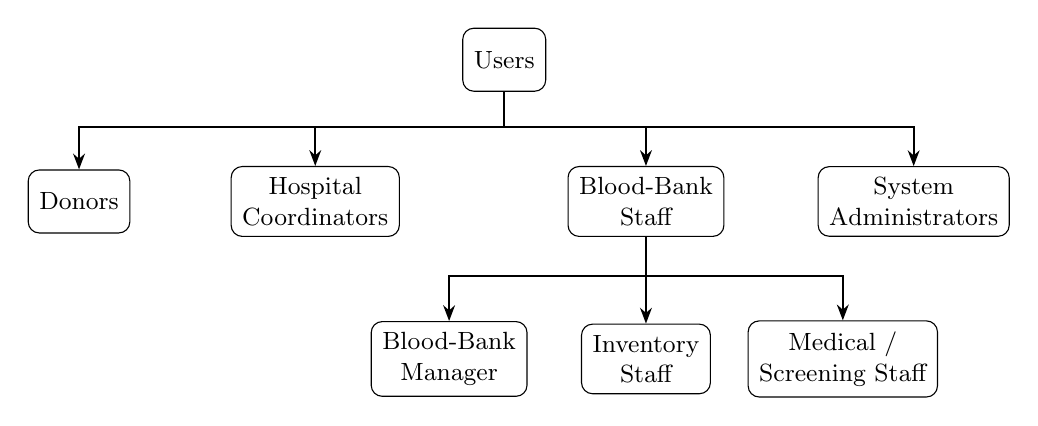
\begin{tikzpicture}[
        n/.style={draw,rounded corners,align=center,font=\small,minimum height=0.8cm,inner sep=4pt},
        l/.style={-{Stealth[length=2mm]},thick}]
        \node[n] (u) at (0,0) {Users};
        \node[n] (d) at (-5.4,-1.8) {Donors};
        \node[n] (h) at (-2.4,-1.8) {Hospital\\ Coordinators};
        \node[n] (s) at (1.8,-1.8) {Blood-Bank\\ Staff};
        \node[n] (a) at (5.2,-1.8) {System\\ Administrators};
        \node[n] (m) at (-0.7,-3.8) {Blood-Bank\\ Manager};
        \node[n] (i) at (1.8,-3.8) {Inventory\\ Staff};
        \node[n] (c) at (4.3,-3.8) {Medical /\\ Screening Staff};
        \draw[l] (u.south) -- ++(0,-0.45) -| (d.north);
        \draw[l] (u.south) -- ++(0,-0.45) -| (h.north);
        \draw[l] (u.south) -- ++(0,-0.45) -| (s.north);
        \draw[l] (u.south) -- ++(0,-0.45) -| (a.north);
        \draw[l] (s.south) -- ++(0,-0.5) -| (m.north);
        \draw[l] (s.south) -- (i.north);
        \draw[l] (s.south) -- ++(0,-0.5) -| (c.north);
    \end{tikzpicture}
    \caption{Type of users}
    \label{fig:users}
\end{figure}
\section{Product Functions}
``BloodLine'' stores the inventory, donors, demand history, forecasts and requests of blood banks. Before using the main functions, users have to be registered.
\newline
All users have - id, email, hashed\_password, full\_name, role, is\_active and created\_at.
\newline
Donors have some extra information - user\_id (foreign key), blood\_group, last\_donation\_date, latitude, longitude, is\_available and notification\_consent.
\newline
Blood banks have - name, address, latitude and longitude. Inventory has blood\_group, component and quantity\_units; every stock change is an inventory transaction (receipt, issue, expiry or discard).
\newline
Demand history has units\_demanded per blood group per day, with an is\_synthetic flag. Predictions and alerts store the forecast, risk\_level, shortfall and explanation.
\newline
Hospital requests have blood\_group, quantity\_units, urgency (routine, urgent, emergency) and status. Screening records have donor, staff member, outcome (eligible, deferred, rejected) and notes.

\begin{figure}[H]
    \centering
    \resizebox{\textwidth}{!}{%
    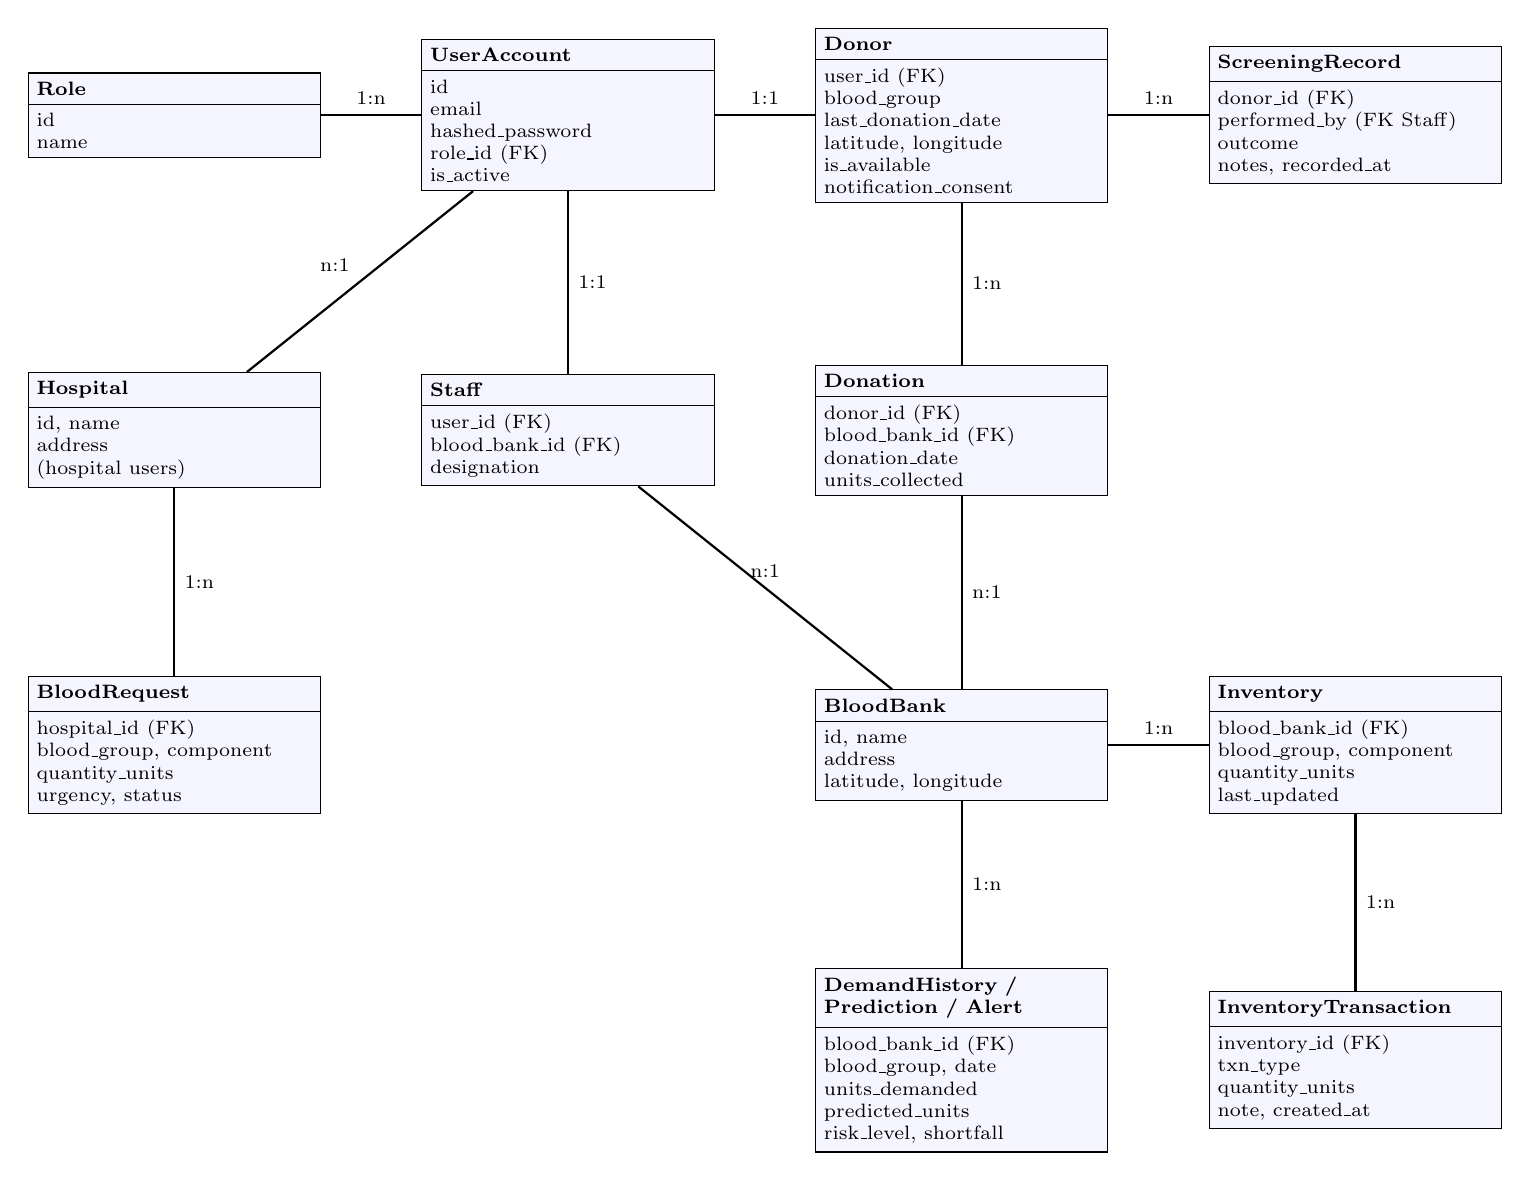
\begin{tikzpicture}[
        ent/.style={draw,rectangle split,rectangle split parts=2,text width=3.5cm,font=\scriptsize,align=left,inner sep=3pt,fill=blue!4},
        rel/.style={thick}]
        \node[ent] (role) at (0,0) {\textbf{Role}\nodepart{second}id\\ name};
        \node[ent] (user) at (5,0) {\textbf{UserAccount}\nodepart{second}id\\ email\\ hashed\_password\\ role\_id (FK)\\ is\_active};
        \node[ent] (donor) at (10,0) {\textbf{Donor}\nodepart{second}user\_id (FK)\\ blood\_group\\ last\_donation\_date\\ latitude, longitude\\ is\_available\\ notification\_consent};
        \node[ent] (screen) at (15,0) {\textbf{ScreeningRecord}\nodepart{second}donor\_id (FK)\\ performed\_by (FK Staff)\\ outcome\\ notes, recorded\_at};
        \node[ent] (hosp) at (0,-4) {\textbf{Hospital}\nodepart{second}id, name\\ address\\ (hospital users)};
        \node[ent] (staff) at (5,-4) {\textbf{Staff}\nodepart{second}user\_id (FK)\\ blood\_bank\_id (FK)\\ designation};
        \node[ent] (don) at (10,-4) {\textbf{Donation}\nodepart{second}donor\_id (FK)\\ blood\_bank\_id (FK)\\ donation\_date\\ units\_collected};
        \node[ent] (req) at (0,-8) {\textbf{BloodRequest}\nodepart{second}hospital\_id (FK)\\ blood\_group, component\\ quantity\_units\\ urgency, status};
        \node[ent] (bank) at (10,-8) {\textbf{BloodBank}\nodepart{second}id, name\\ address\\ latitude, longitude};
        \node[ent] (inv) at (15,-8) {\textbf{Inventory}\nodepart{second}blood\_bank\_id (FK)\\ blood\_group, component\\ quantity\_units\\ last\_updated};
        \node[ent] (fc) at (10,-12) {\textbf{DemandHistory /\\ Prediction / Alert}\nodepart{second}blood\_bank\_id (FK)\\ blood\_group, date\\ units\_demanded\\ predicted\_units\\ risk\_level, shortfall};
        \node[ent] (txn) at (15,-12) {\textbf{InventoryTransaction}\nodepart{second}inventory\_id (FK)\\ txn\_type\\ quantity\_units\\ note, created\_at};
        \draw[rel] (role)--(user) node[midway,above,font=\scriptsize]{1:n};
        \draw[rel] (user)--(donor) node[midway,above,font=\scriptsize]{1:1};
        \draw[rel] (donor)--(screen) node[midway,above,font=\scriptsize]{1:n};
        \draw[rel] (user)--(hosp) node[midway,above left,font=\scriptsize]{n:1};
        \draw[rel] (user)--(staff) node[midway,right,font=\scriptsize]{1:1};
        \draw[rel] (donor)--(don) node[midway,right,font=\scriptsize]{1:n};
        \draw[rel] (hosp)--(req) node[midway,right,font=\scriptsize]{1:n};
        \draw[rel] (don)--(bank) node[midway,right,font=\scriptsize]{n:1};
        \draw[rel] (staff)--(bank) node[midway,above,font=\scriptsize]{n:1};
        \draw[rel] (bank)--(inv) node[midway,above,font=\scriptsize]{1:n};
        \draw[rel] (bank)--(fc) node[midway,right,font=\scriptsize]{1:n};
        \draw[rel] (inv)--(txn) node[midway,right,font=\scriptsize]{1:n};
    \end{tikzpicture}}
    \caption{Data model (main entities and relations)}
    \label{fig:data}
\end{figure}
Alert is the main feature of all. It combines the stock of a blood group with its forecast and shows the manager the level, the shortfall and the reason.

\section{Operating Environment}
The website will be operated in any Operating Environment - Mac, Windows, Linux, Android, iOS etc. - through a modern web browser. The backend runs on common web hosting with a managed database. The interface is responsive, so low-to-mid range devices can use it. Where real consumption data is not available, clearly labelled simulated data is used.

\section{Design}
Donor activities have 3 steps - Registration and Profile, Availability and Consent, Alerts and Donation History. Activities of the other roles are shown in Figure~\ref{fig:roles}.

\begin{figure}[H]
    \centering
    \resizebox{\textwidth}{!}{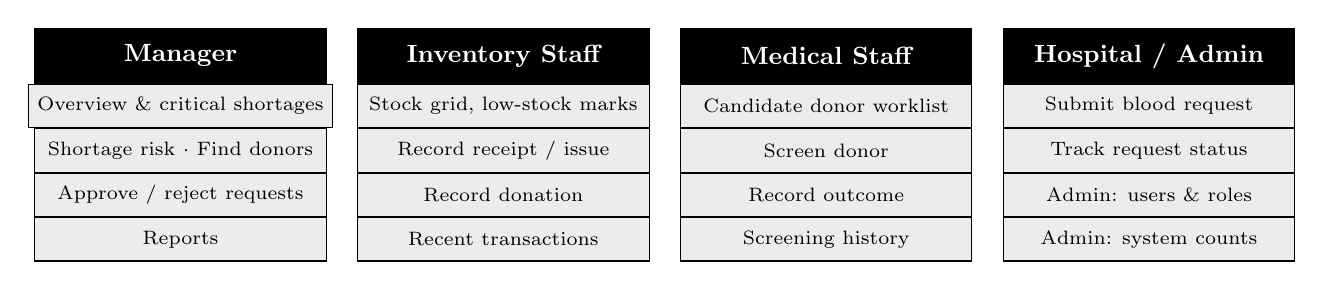
\begin{tikzpicture}[
        hd/.style={draw,fill=black,text=white,font=\small\bfseries,minimum width=3.7cm,minimum height=0.7cm,align=center},
        it/.style={draw,fill=gray!15,font=\scriptsize,minimum width=3.7cm,minimum height=0.55cm,align=center}]
        % columns
        \node[hd] at (0,0) (m) {Manager};
        \node[it,below=0pt of m] (m1) {Overview \& critical shortages};
        \node[it,below=0pt of m1] (m2) {Shortage risk $\cdot$ Find donors};
        \node[it,below=0pt of m2] (m3) {Approve / reject requests};
        \node[it,below=0pt of m3] (m4) {Reports};
        \node[hd] at (4.1,0) (i) {Inventory Staff};
        \node[it,below=0pt of i] (i1) {Stock grid, low-stock marks};
        \node[it,below=0pt of i1] (i2) {Record receipt / issue};
        \node[it,below=0pt of i2] (i3) {Record donation};
        \node[it,below=0pt of i3] (i4) {Recent transactions};
        \node[hd] at (8.2,0) (c) {Medical Staff};
        \node[it,below=0pt of c] (c1) {Candidate donor worklist};
        \node[it,below=0pt of c1] (c2) {Screen donor};
        \node[it,below=0pt of c2] (c3) {Record outcome};
        \node[it,below=0pt of c3] (c4) {Screening history};
        \node[hd] at (12.3,0) (h) {Hospital / Admin};
        \node[it,below=0pt of h] (h1) {Submit blood request};
        \node[it,below=0pt of h1] (h2) {Track request status};
        \node[it,below=0pt of h2] (h3) {Admin: users \& roles};
        \node[it,below=0pt of h3] (h4) {Admin: system counts};
    \end{tikzpicture}}
    \caption{Role-wise activities of staff, hospital and admin users}
    \label{fig:roles}
\end{figure}
Manager can review the risk, find donors, and approve or reject requests. Inventory staff record stock and donations. Medical staff only screen donors. Hospital coordinator only creates and tracks requests. Administrator only manages accounts.

\chapter{System Features}
``BloodLine'' is a predictive blood-availability web software. So the main art of this product is to keep stock correct, forecast demand, detect shortage risk early and match donors.

\section{Description and Priority}
``BloodLine'' has features that are main and also some are sub. But all the features are necessary for this software.
\newline
The features with priority up to down -
\begin{enumerate}
    \item Inventory Tracking : The base of all. Operated by inventory staff. \hfill MVP
    \item Demand Forecasting : Estimates near-term demand of every blood group. \hfill MVP
    \item Shortage-Risk Detection : Compares forecast with stock and flags risk. This is the goal feature. \hfill MVP
    \item Smart Donor Matching : Suggests compatible, available and consenting donors. \hfill MVP
    \item Role-Based Access : Separate pages and permissions for the six roles. \hfill MVP
    \item Hospital Requests : Request, approval and automatic issue of stock. \hfill Inc.\,2
    \item Screening Workflow : Medical staff clear donors and record outcomes. \hfill Inc.\,2
    \item Notifications : Alerts only to matched donors. \hfill Inc.\,2
    \item Reports and Regional View : Summaries and heatmap of surplus and shortage. \hfill Inc.\,2
\end{enumerate}

\section{Functional Requirements}
Each requirement has an ID (FR-xxx-n), a ``shall'' statement and the increment (\textbf{M} = MVP, \textbf{2} = Inc.\,2).

\subsection*{Authentication and Access (AUTH)}
\begin{longtable}{@{}l L{11.6cm} l@{}}
\toprule
\textbf{ID} & \textbf{Requirement} & \textbf{Inc.}\\
\midrule
\endhead
FR-AUTH-1 & The system shall let a registered user log in with email and password; passwords are stored only as salted hashes. & M\\
FR-AUTH-2 & On login the system shall issue a signed token with the user's role, which expires after a fixed time (default 8 hours). & M\\
FR-AUTH-3 & The system shall deny any request without a valid token or from a role that is not authorised, and shall block deactivated accounts. & M\\
FR-AUTH-4 & A donor shall be able to self-register with blood group, approximate location and consent. & 2\\
\bottomrule
\end{longtable}

\subsection*{Inventory (INV)}
\begin{longtable}{@{}l L{11.6cm} l@{}}
\toprule
\textbf{ID} & \textbf{Requirement} & \textbf{Inc.}\\
\midrule
\endhead
FR-INV-1 & The system shall keep current stock (units) per blood bank, blood group and component. & M\\
FR-INV-2 & Inventory staff shall record receipt, issue, expiry or discard with quantity and note; every transaction is timestamped and logged. & M\\
FR-INV-3 & The system shall reject zero or negative quantities and any issue larger than the units available. & M\\
FR-INV-4 & The dashboard shall mark blood groups below a low-stock level (default 15 units). & M\\
FR-INV-5 & A recorded donation shall update the donor's last donation date and increase the stock. & M\\
FR-INV-6 & The system shall track single units with collection and expiry date and flag units close to expiry. & 2\\
\bottomrule
\end{longtable}

\subsection*{Demand Forecasting (FCST)}
\begin{longtable}{@{}l L{11.6cm} l@{}}
\toprule
\textbf{ID} & \textbf{Requirement} & \textbf{Inc.}\\
\midrule
\endhead
FR-FCST-1 & The system shall store daily demand per blood group; simulated data shall carry an is\_synthetic flag and be labelled ``Synthetic / Simulated'' on every screen. & M\\
FR-FCST-2 & The system shall forecast near-term demand (default 7 days) of every blood group using a time-series model (Prophet or SARIMA in the final system). & M\\
FR-FCST-3 & Every forecast shall be compared with a naive moving-average baseline and shall report the model used, the predicted units and the error. & M\\
FR-FCST-4 & Data shall be split chronologically into training and test periods, and MAE and RMSE computed on the test period. & M\\
FR-FCST-5 & The model shall be replaceable without changing the API, and the data layer shall accept authorized real data. & 2\\
\bottomrule
\end{longtable}

\subsection*{Shortage Risk (RISK)}
Shortfall = forecast demand $-$ current stock.
\begin{longtable}{@{}l L{11.6cm} l@{}}
\toprule
\textbf{ID} & \textbf{Requirement} & \textbf{Inc.}\\
\midrule
\endhead
FR-RISK-1 & The system shall classify risk as \textbf{LOW} if shortfall $\le$ 0; \textbf{MODERATE} if 0 $<$ shortfall $\le$ 25\% of stock; \textbf{HIGH} if shortfall $>$ 25\% of stock, or if stock is zero and demand is expected. Thresholds are configurable. & M\\
FR-RISK-2 & Every result shall carry a plain-English explanation (stock, forecast, shortfall, reason); the rule layer is transparent, not a black box. & M\\
FR-RISK-3 & Alerts shall be stored with level, shortfall and timestamp, and the manager's overview shall list critical shortages with a ``Find donors'' action. & M\\
\bottomrule
\end{longtable}
Example: 20 units in stock and 25 forecast gives shortfall 5, which is 25\% of stock, so MODERATE.

\subsection*{Donor Matching (MATCH)}
\begin{longtable}{@{}l L{11.6cm} l@{}}
\toprule
\textbf{ID} & \textbf{Requirement} & \textbf{Inc.}\\
\midrule
\endhead
FR-MATCH-1 & For a target blood group the system shall include only compatible donor groups (table below). & M\\
FR-MATCH-2 & The system shall exclude donors who are unavailable, have not given consent, or donated within the cooldown (default 90 days). & M\\
FR-MATCH-3 & The system shall filter donors by distance within a configurable radius. & 2\\
FR-MATCH-4 & Candidates shall be ranked by a score (exact group match, longer time since last donation, nearness), each with reasons. & M\\
FR-MATCH-5 & Results shall be shown as candidates to contact; the system shall never declare a donor medically eligible. & M\\
\bottomrule
\end{longtable}
\begin{center}
\small
\begin{tabular}{@{}ll@{\qquad}ll@{}}
\toprule
\textbf{Patient} & \textbf{Compatible donors} & \textbf{Patient} & \textbf{Compatible donors}\\
\midrule
O$-$ & O$-$ & O+ & O$-$, O+\\
A$-$ & O$-$, A$-$ & A+ & O$-$, O+, A$-$, A+\\
B$-$ & O$-$, B$-$ & B+ & O$-$, O+, B$-$, B+\\
AB$-$ & O$-$, A$-$, B$-$, AB$-$ & AB+ & all eight groups\\
\bottomrule
\end{tabular}
\end{center}

\subsection*{Requests, Screening, Notifications, Reports (Inc.\,2)}
\begin{longtable}{@{}l L{11.6cm} l@{}}
\toprule
\textbf{ID} & \textbf{Requirement} & \textbf{Inc.}\\
\midrule
\endhead
FR-REQ-1 & A hospital coordinator shall submit a request (group, quantity, urgency, notes) and see only the own hospital's requests. & 2\\
FR-REQ-2 & On approval the system shall issue the units from stock and set the status \emph{fulfilled}; if stock is not enough the request stays \emph{pending} with a note. The manager can also reject. & 2\\
FR-SCR-1 & Medical staff shall see a worklist of candidate donors and record the outcome (eligible, deferred, rejected) with notes. The outcome is always entered by a person, never automatically. & 2\\
FR-NOTE-1 & The system shall send in-app/push alerts only to donors who satisfy the matching rules, store them, and stop when consent is withdrawn. & 2\\
FR-RPT-1 & The manager shall view reports of units received, issued and expired, risk summary and demand versus forecast; reports shall be exportable. & 2\\
FR-REG-1 & The system shall show a regional heatmap of surplus and shortage across blood banks to help coordination. & 2\\
\bottomrule
\end{longtable}

\subsection*{Donor Portal and Administration (MVP)}
\begin{longtable}{@{}l L{11.6cm} l@{}}
\toprule
\textbf{ID} & \textbf{Requirement} & \textbf{Inc.}\\
\midrule
\endhead
FR-DON-1 & A donor shall view own profile, eligibility status and donation history, and switch availability and consent. & M\\
FR-ADM-1 & The administrator shall view system counts and users, create and deactivate accounts, and assign roles. & M\\
FR-ADM-2 & The system shall write basic logs with timestamps for logins, stock changes and admin actions. & M\\
\bottomrule
\end{longtable}

\subsection*{Technology Stack}
The ``BloodLine'' website is being built on React, Tailwind CSS, FastAPI (Python), PostgreSQL and Pandas with statsmodels/Prophet.
\newline
Front-End - React.js, Tailwind CSS, JavaScript.
\newline
Back-End - FastAPI (Python), REST API.
\newline
Database - PostgreSQL.
\newline
Forecasting - Pandas, statsmodels, Prophet. Maps - Google Maps API or equivalent.

\chapter{Other Nonfunctional Requirements}

\section{Performance Requirements}
``BloodLine'' will be used in daily work of blood banks, so common actions must be quick. Targets for up to 50 concurrent users: inventory update $\le$ 1 s, dashboard loading $\le$ 3 s, donor search $\le$ 2 s. For growth, the backend is stateless, frontend and backend are decoupled, and large lists use pagination and database indexes.

\section{Security Requirements}
No one without registered users can enter the website. One particular user of a role only can perform his/her particular actions.
\begin{itemize}
    \item Passwords are stored as salted hashes; sessions use signed, expiring tokens; all traffic uses HTTPS.
    \item Role checks are done on the server for every protected request.
    \item A donor sees only own data; a hospital coordinator sees only own hospital's requests.
    \item Personal data is minimised, and alerts go only to consenting donors who satisfy the matching rules.
\end{itemize}

\section{Software Quality Attributes}
In the development phase also testing and conferences of users is continued, so that the quality of the software is maintained and all the requirements are fulfilled. Database, logical and also UI test is required. Success is measured by:
\begin{center}
\small
\begin{tabularx}{\textwidth}{@{}l X@{}}
\toprule
\textbf{Metric} & \textbf{How it is measured}\\
\midrule
Forecasting error (primary) & MAE and RMSE of predicted versus actual demand in the held-out test period\\
Shortage-risk performance & Known shortage cases in test data are correctly flagged\\
Donor-matching correctness & Seeded donors check that group, cooldown, proximity, availability and consent filters work\\
Workflow response time & Time of inventory update, dashboard load and donor search\\
Notification targeting & Alerts reach only donors who satisfy the matching rules\\
\bottomrule
\end{tabularx}
\end{center}
Other attributes: stock never becomes negative; every risk level and match has a readable reason; forecasting, risk and matching are separate modules, so a model can be swapped; the build runs automated unit tests and linting on every change.

\section{Business Rules}
``BloodLine'' is for finding and preventing blood shortages early. Basically save working time and pressure.
\begin{itemize}
    \item Final donor clearance is given only by qualified medical staff.
    \item Actual movement of blood between banks remains with authorized staff.
    \item A donor is contacted only if compatible, available, consenting and past cooldown.
    \item A request is fulfilled only if enough stock exists.
    \item Simulated data is never presented as real data; forecasts always get human review.
\end{itemize}

\chapter{Other Requirements}
``BloodLine'' needs maintenance as it is a long process software. It will need re-factoring and further the requirements can be changed as the field is changing frequently. CI/CD will build and test every change automatically and deploy to staging, so features are released in weekly iterations. Main risks are handled as - unavailable real data: use labelled simulated data and keep the data layer ready for real data; forecast uncertainty: show risk signals with human review; medical and privacy limits: staff do final clearance and access is by role.

\end{document}
